\documentclass{article}
\usepackage{graphicx,amsmath,amssymb,url,multirow}
\usepackage{hyperref}
% \usepackage{wrapfig}
\usepackage[nottoc,numbib]{tocbibind}
\usepackage{booktabs}
\setlength{\parindent}{0.0in}
\setlength{\parskip}{0.07in}

%\usepackage[paper=a4paper,dvips,top=1.5cm,left=1.5cm,right=1.5cm,
%    foot=1cm,bottom=1.5cm]{geometry}
\usepackage[paper=a4paper,top=3cm,left=2cm,right=2cm,bottom=3cm]{geometry}

% TITLE
\title{Low-Fi Validation Report}
\author{Version 0.1 Beta}
\date{Copyright \textcircled{c}  2014 Sigma Power Engineering Pty Ltd}

\begin{document}
\pagestyle{plain}
\maketitle

% TABLE OF CONTENTS
\tableofcontents
\clearpage

% BODY
\section{Introduction}
\subsection{About Low-fi}
\textbf{Low-fi} is a simulation tool for calculating the low frequency induction (LFI) effects between an overhead powerline and a pipeline sharing a joint right-of-way. Specifcally, \textbf{Low-fi} computes the induced voltages along the length of a pipeline relative to earth (the so-called \emph{pipeline-to-earth touch voltage} or \emph{shunt potential}), which is relevant for the analysis of personnel safety.

Refer also to the \textbf{Low-fi} user documentation for details on how the simulation results are calculated and general software handling. 

\subsection{About Sigma Power Engineering}
%\begin{wrapfigure}{l}{0.3\textwidth}
%  \begin{center}
\begin{figure}[!ht]
    
\includegraphics[width=0.28\textwidth]{./Figures/Sigma_Power.png}
\end{figure}

%  \end{center}
%\end{wrapfigure}

\textbf{Sigma Power Engineering Pty Ltd} is an electrical engineering consultancy and software developer based in Perth, Australia.

We are a small team of power systems engineers with broad experience in the utility, hydrocarbons and mining sectors of Australia, Asia and Europe. Our primary focus is to offer the full range of power system studies services, while also supporting our clients with our software tools, project management and design engineering capabilities.

For more details, visit our website \href{http://www.sigmapower.com.au}{www.sigmapower.com.au}.

\subsection{Scope of Report}
In this report, \textbf{Low-fi} is used on a number of case studies to simulate load and fault LFI voltages. The simulation results are then compared to other software packages (e.g. CDEGS and PRC) as well as measured data, in order to validate \textbf{Low-fi} and articulate its limitations. All of the case studies presented in this report can be found in the Examples directory of \textbf{Low-fi} for verification by the user.

\newpage
\section{Simple Right-of-Way}
A case study showing a simple right-of-way is presented first. The right-of-way has a single-circuit overhead line running in parallel with a straight section of buried pipeline with equal earthing resistances at each end. Key parameters such as separation distance, parallel exposure length, pipeline end earthing resistance and soil resistivity are altered and the resulting fault LFI voltages are compared with with simulations performed in CDEGS software.

The case study has the following base parameters:
\begin{itemize}
\item The overhead line tower geometry is as per Figure \ref{fig:simple_geo}. The earth wire has impedance $Z_{w} = 0.2741 + j0.2406 \Omega$/km. 
\item The pipeline is a 24" line with metal resistivity of $1.68 \times 10^{-7} \Omega.m$ and relative permeability of 300.
\item The pipeline coating is 1" thick with a coating resistivity of $5 \times 10^{7} \Omega.m$ and relative permeability of 1. 
\item The pipeline is earthed at each end to resistive earth grids (resistances to be varied during the study)
\item The system has a nominal frequency of 50Hz and a prospective earth fault current of 40kA, where it is assumed that 90\% of the fault current flows through the earth. 
\end{itemize}

\begin{figure}[!htp]
\begin{center}
\caption{Tower geometry for simple right-of-way}
\label{fig:simple_geo}
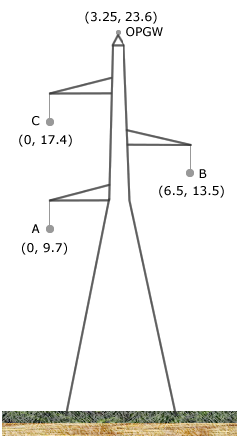
\includegraphics[width=0.35\linewidth]{./Figures/simple_geo.png}
\end{center}
\end{figure}

In the base case, the following parameters are used:
\begin{itemize}
\item Parallel exposure length = 6km
\item Separation distance = 100m
\item Pipeline end earthing resistances = 0.1$\Omega$
\item Soil resistivity = 100$\Omega.m$
\end{itemize} 

Figure \ref{fig:simple_cdegs} shows the simulation results of the base case in \textbf{Low-fi} and CDEGS. It can be seen that the shape of the induced voltages are identical, but there are minor differences in the induced voltages at the pipeline ends.

\begin{figure}[!htp]
\begin{center}
\caption{Comparison of base case results with CDEGS}
\label{fig:simple_cdegs}
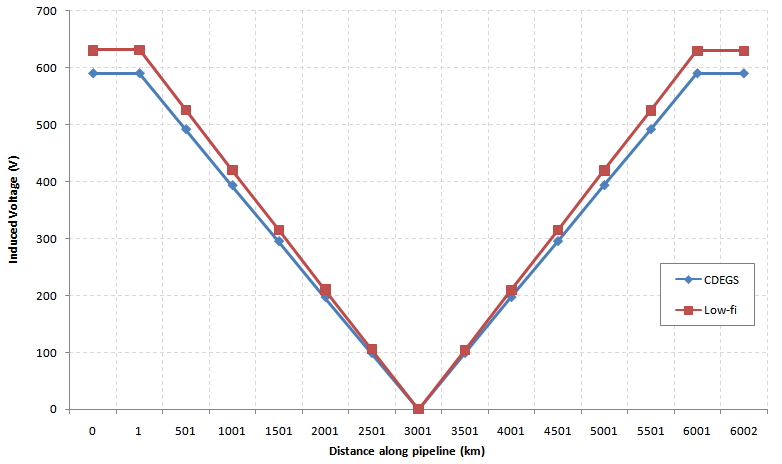
\includegraphics[width=0.8\linewidth]{./Figures/simple_cdegs.png}
\end{center}
\end{figure}

Ten variations on the parameters of the simple right-of-way are made and the \textbf{Low-fi} simulation results are compared against results from CDEGS. A summary of the comparison is shown in Table \ref{tab:simple_cdegs} below.

\begin{table}[!htp]
\caption{Comparison of \textbf{Low-fi} results with CDEGS for variations on simple right-of-way parameters}
\label{tab:simple_cdegs}
\begin{tabular}{@{}ccccccccc@{}}
\toprule
\multirow{3}{*}{\textbf{Case}} \\& \textbf{Exposure}  & \textbf{Separ-} & \textbf{Soil} & \textbf{Earth}  & \multicolumn{3}{c}{\textbf{Simulated Induced Voltage (V)}} & \textbf{Max Separ-} \\ \cmidrule(lr){6-8}
& \textbf{Length} & \textbf{ation (m)} & \textbf{Rho ($\Omega$.m)} &  \textbf{Resistance}                                                      & \textbf{CDEGS}   & \textbf{Low-fi}   & \textbf{\parbox{0.1\textwidth}{Deviation}}  &  \textbf{ation (m)}  \\
& \textbf{(km)} &  &  &  \textbf{($\Omega$)} &   &   &   &                                       \\ \midrule
Base                              & 6                                              & 100                                      & 100                                                & 0.1                                                    & 590              & 630               & 6.78\%              & 127                                              \\ \midrule
1                              & 6                                              & 270                                      & 100                                                & 0.4                                                    & 1390             & 1472              & 5.90\%              & 127                                              \\ \midrule
2                              & 6                                              & 350                                      & 100                                                & 0.4                                                    & 1180             & 1261              & 6.86\%              & 127                                              \\ \midrule
3                              & 6                                              & 500                                      & 100                                                & 0.4                                                    & 900              & 1008              & 12.00\%             & 127                                              \\ \midrule
4                              & 12                                             & 480                                      & 100                                                & 0.4                                                    & 1000             & 1072              & 7.20\%              & 127                                              \\ \midrule
5                              & 6                                              & 250                                      & 20                                                 & 0.4                                                    & 950              & 989               & 4.11\%              & 57                                               \\ \midrule
6                              & 6                                              & 450                                      & 20                                                 & 0.4                                                    & 500              & 852               & 70.40\%             & 57                                               \\ \midrule
7                              & 3                                              & 300                                      & 100                                                & 0.4                                                    & 1190             & 1239              & 4.12\%              & 127                                              \\ \midrule
8                              & 3                                              & 400                                      & 100                                                & 0.4                                                    & 970              & 1039              & 7.11\%              & 127                                              \\ \midrule
9                             & 1                                              & 100                                      & 100                                                & 0.4                                                    & 1275             & 1277              & 0.16\%              & 127                                              \\ \midrule
10                             & 1                                              & 200                                      & 100                                                & 0.4                                                    & 950              & 939               & -1.16\%             & 127                                              \\ \bottomrule
\end{tabular}
\end{table}

The \textbf{Low-fi} and CDEGS results are generally within 6\%, with the \textbf{Low-fi} simulations being slightly more conservative in the majority of cases. 

An important observation is that \textbf{Low-fi} accuracy falls off significantly for Case 6, with a 70\% deviation from the CDEGS results. This is due to the limitations of the AS 4853 (or Carson-Clem) formulation for mutual impedance between the overhead line and buried pipeline. As noted in the \textbf{Low-fi} user documentation, this formulation is accurate for separation distances less than $90 \sqrt{\frac{\rho}{f}}$.

The last column of Table \ref{tab:simple_cdegs} shows the maximum separation distance for each case. It can be seen that when the separation distances deviate too far from the maximum distance, the error becomes larger (for example, the separation distance in Case 6 is 7.9 times larger than the maximum allowable distance).

\newpage
\section{Kalamazoo Line 1800}
The original case study for the Consumers Power Company line 1800 pipeline in Kalamazoo is described on page 3-51 of EPRI report EL-904 \cite{EPRI_1978}. The pipeline is a 20" gas line located near Kalamazoo, Michigan, running for approximately 31.1km from the Plainwell valve site in the south (0km) to the 30th street valve site in the north (31.1km). The pipeline shares a joint right-of-way with a 345kV overhead tower line, which runs in parallel with the pipeline for approximately 27.1km. A cross-sectional layout of the joint right-of-way is shown in Figure \ref{fig:kalamazoo_geo}. 

\begin{figure}[!htp]
\begin{center}
\caption{Tower and pipeline geometry for Kalamazoo line 1800 \cite{EPRI_1978}}
\label{fig:kalamazoo_geo}
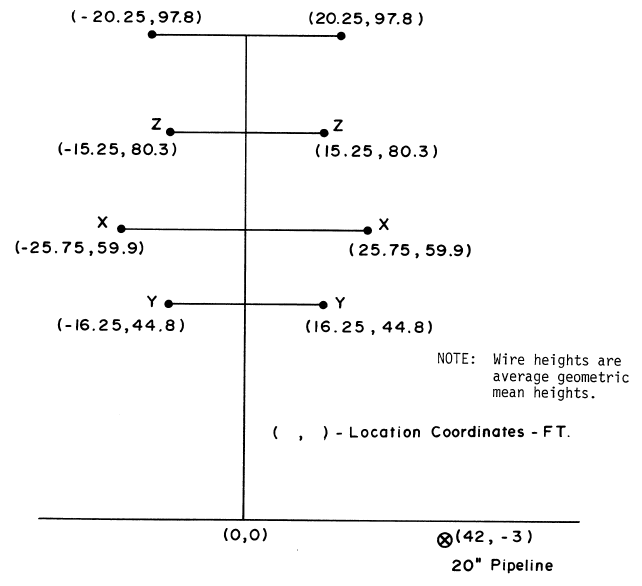
\includegraphics[width=0.8\linewidth]{./Figures/kalamazoo_geo.png}
\end{center}
\end{figure}

Data entry and assumptions for the case study are as follows:
\begin{itemize}
\item \textbf{Earthing resistances}: at the Plainwell valve site (0km), the earthing resistance was measured to be 0.15$\Omega$. At the 30th street valve site (31.1km), the pipeline is physically connected to a 24" pipeline (with different coating characteristics) and then bonded to another 16" pipeline. The equivalent earthing impedance of these pipelines is calculated to be 0.4 + j0.314 $\Omega$. \textbf{Low-fi} only supports real earthing impedances and so the magnitude of the equivalent impedance is used (0.44$\Omega$).
\item \textbf{Pipeline characteristics}: line 1800 is a 20" buried pipeline with (a) pipe steel resistivity = 0.17 $\mu\Omega$.m, (b) pipe steel relative permeability = 300, (c) coating resistivity = 300,000 $\Omega.ft^{2}$ = $2.787 \times 10^{7} \Omega$.m
\item \textbf{Soil resistivity}: 400 $\Omega$.m
\item \textbf{Tower characteristics}: the tower geometry is as per Figure \ref{fig:kalamazoo_geo}. Note that a double-circuit tower is shown in the figure. In \textbf{Low-fi}, this is converted to a single-circuit tower by taking the mean positions of the phase and earth conductors.
\item \textbf{Network characteristics}: the network is a 60Hz system and the load current is 50A (balanced).
\end{itemize}

The validation results for load LFI on line 1800 are shown in Figure \ref{fig:kalamazoo_comparison}, with comparisons to measured data, CDEGS simulation results and PRC simulation results.

\begin{figure}[!htp]
\begin{center}
\caption{\textbf{Low-fi} validation results for Kalamazoo line 1800}
\label{fig:kalamazoo_comparison}
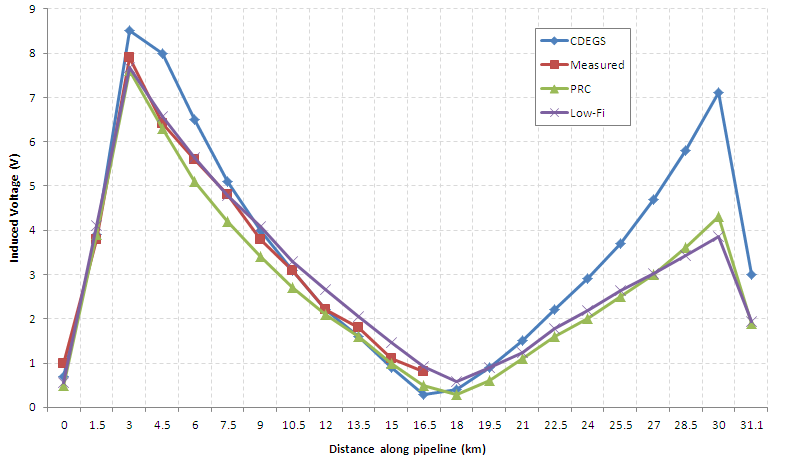
\includegraphics[width=\linewidth]{./Figures/kalamazoo_comparison.png}
\end{center}
\end{figure}

The following observations are made regarding the validation results:
\begin{itemize}
\item There is generally very good agreement between the results from \textbf{Low-fi} and the results from measurements and other software packages.
\item Like \textbf{Low-fi}, PRC only supports real earthing resistances, which explains the deviation from the CDEGS results at the 30th street end (31.1km). 
\end{itemize}

\newpage
\section{Needles Line 235}
The Southern California Gas Company pipeline 235 shares a right-of-way with a Southern California Edison 500kV overhead transmission line for approximately 52 miles near Needles, California in the Mojave desert. A plan layout of the joint right-of-way is shown in Figure \ref{fig:needles_row} and the tower geometry is shown in Figure \ref{fig:needles_geo}. 

\begin{figure}[!htp]
\begin{center}
\caption{Right-of-way for Needles line 235 \cite{taflove_1979}}
\label{fig:needles_row}
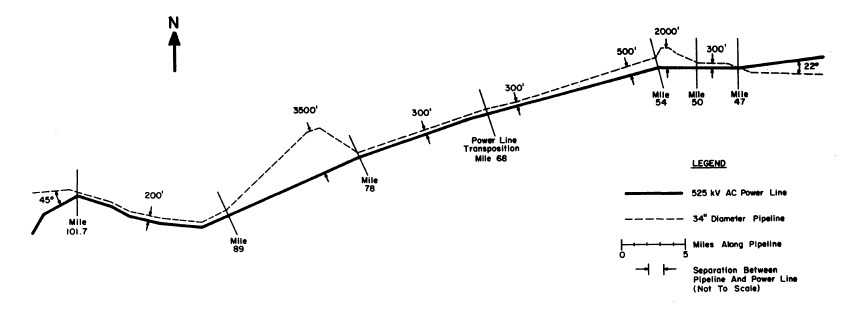
\includegraphics[width=\linewidth]{./Figures/needles_row.png}
\end{center}
\end{figure}

\begin{figure}[!htp]
\begin{center}
\caption{Tower geometry for Needles line 235 \cite{taflove_1979}}
\label{fig:needles_geo}
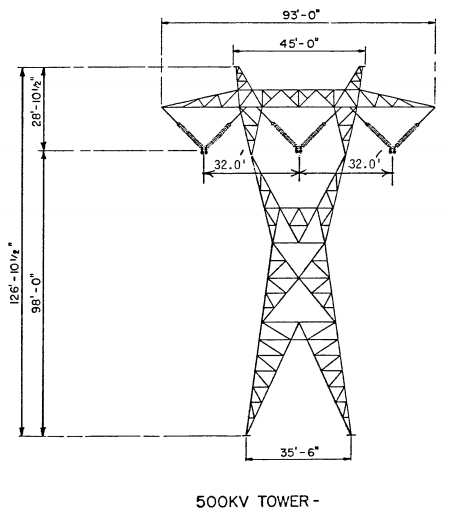
\includegraphics[width=0.4\linewidth]{./Figures/needles_geo.png}
\end{center}
\end{figure}

Data entry and assumptions for the case study are as follows:
\begin{itemize}
\item \textbf{Earthing resistances}: there is no information on pipeline earthing, so no earthing resistances are modelled. 
\item \textbf{Pipeline characteristics}: line 235 is a 34" buried gas transmission line running from Newberry to Needles, California, with (a) pipe steel resistivity = 0.17 $\mu\Omega$.m (assumed), (b) pipe steel relative permeability = 300 (assumed), (c) coating resistivity = 700,000 $\Omega.ft^{2}$ = $6.5 \times 10^{7} \Omega$.m
\item \textbf{Soil resistivity}: 400 $\Omega$.m
\item \textbf{Tower characteristics}: the tower geometry is as per Figure \ref{fig:needles_geo} and there is a phase-wise transposition at Milepost 68.
\item \textbf{Network characteristics}: the network is a 60Hz system and the load current is 700A (balanced).
\end{itemize}

The validation results for load LFI on Needles line 235 are shown in Figure \ref{fig:needles_comparison}, with comparisons to measured data, CDEGS simulation results and PRC simulation results.

\begin{figure}[!htp]
\begin{center}
\caption{\textbf{Low-fi} validation results for Needles line 235}
\label{fig:needles_comparison}
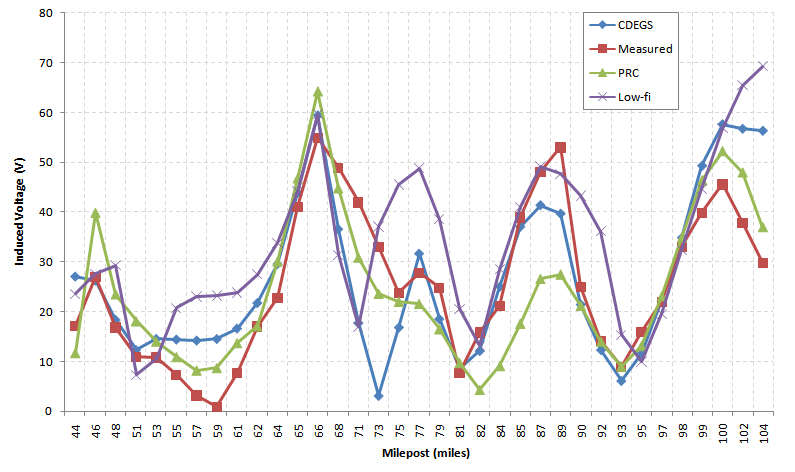
\includegraphics[width=\linewidth]{./Figures/needles_comparison.png}
\end{center}
\end{figure}

The following observations are made regarding the validation results:
\begin{itemize}
\item The results from \textbf{Low-fi} are able to predict the voltage peaks on the pipeline and compare quite well with the measurements and results from other software packages.
\item \textbf{Low-fi} results are generally more conservative than the other software packages, for example, predicting a larger peak at milepost 77. 
\item The large peak at milepost 77 can be attributed to the fact that the separation distances in this area are quite large (3000ft = 914m). The maximum separation distance for which the Carson-Clem equations are accurate is in the order of 255m, which helps to explains the inaccuracy. The same logic applies for the area between mileposts 50 and 57, where the \textbf{Low-fi} results deviate from the other results due to the higher separation distances (up to 2000ft = 610m).
\item Earthing resistances at the ends of the pipeline were not known and therefore not modelled. This has the effect of pushing the voltage up at the ends of the pipeline, particularly at milepost 104.
\end{itemize}

\newpage
% Bibliography
\bibliographystyle{plain}
\bibliography{bib_refs}

\end{document}
